\section{Measurement Method}
For the time measurements, we can implement a simulation program that will record the elapsed time of a running software updates protocol executed by $u$ active users.

\subsection{Benchmarking Data}
The existing benchmarking data try to create an artificial load in order to
stress test the performance of the nodes. The tweakable parameters of the benchmarks are:

\begin{description}
  \item \textbf{generators} the number of processes which are
    responsible for transaction generation.
  \item \textbf{conc} the number of threads that a generator spawns to create
    the actual transactions
  \item \textbf{txs/thread} the number of transactions that an individual thread
    is going to create during a benchmark.
  \item \textbf{delay} time that a thread waits before issuing the next
    transaction.
\end{description}

Roughly, benchmarking architecture works as follows:
The generators (running on the same machine) issue transactions and send them
to unprivileged. Unprivileged relays function as nodes running the protocol and
forward these transactions to a number of privileged nodes, which then in turn
send them to the core nodes in order to issue the blocks. In the current setup
there are 3 unprivileged nodes, and 7 privileged. We can't  however scale
the number of unprivileged or privileged to a high number as each of these is an
AWS instance.

The total number or transactions is $generators * conc * txs/thread$.
It's good to have in mind that we can change the delay, although it is used
as a way to stress the system more in the benchmarks, while in our case we might
want to see how the system may behave in a longer timeframe. I don't think it
is a useful parameter to think of now, as it complicates things, but good to
know that it exists.

\begin{itemize}

  \item we can calculate the number of users indirectly. We have a total number
of transactions, $tx$, so if we want to simulate n users, we will assume a rate
of $\frac{tx}{n}$ per user.
  \item Another less artificial approach would be to rerun the benchmarks for
different sizes of $conc$ and $generators$, and safely assume that $users$ =
    $conc * generators$. The benchmarking data available use a small conc (1 and
    2) which cannot scale effectively, so increasing the generators is the only
    option to proceed. However the current setup runs all generators on the same
    machine, so it not possible to scale them as well. After discussions with
    the benchmarking team, the best way to simulate the number of users is using
    a high number of unprivileged nodes, which is impractical as each node is
    a seperate instance.

\end{itemize}
The KPI measured which are relevant to us is \textbf{tx submission time},
\begin{description}
  \item \textbf{Tx Submission Time} Following the second approach, this
    is the TST for a number of $n = conc * generators$ users.

\end{description}

\begin{figure}[h!]
    \caption{The lifecycle of a software update (a decentralized approach)}
    \centering
    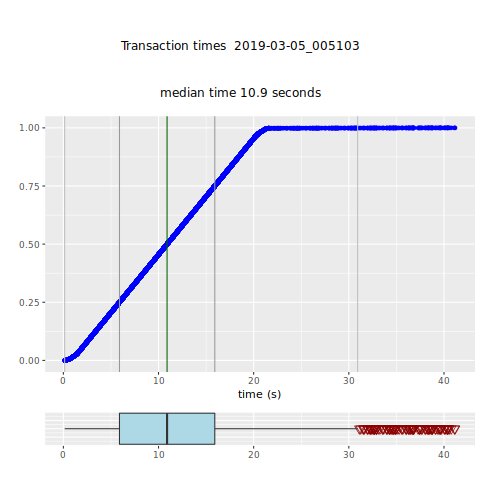
\includegraphics[width=\textwidth]{figures/tst.png}
   % 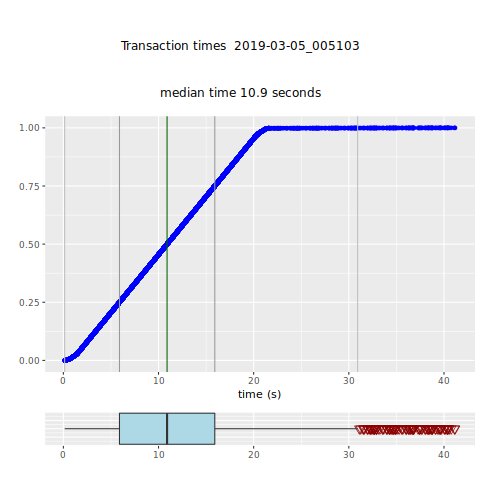
\includegraphics[width=1.0 \columnwidth,keepaspectratio]{figures/tst.png}
    \label{tst}
\end{figure}


We know we can freely parse the trace data in different ways depending on our
target $n$, is this the same with the benchmarking data? If yes, its easier to
follow the first approach, if the answer is no, we should run benchmarks with
different parameter sets, which as detailed above is not something we can do
easily.

Concluding, the most versatile approach is to use the distribution from a high
load benchmark like \ref{tst}, which practically comes down to sampling from a
uniform 0-20 sec distribution for TST.

\subsection{Update Protocol}
The numbers of users $n$ refers to the users running the protocol. We assume
$m$ proposals, and each transaction belonging to the same UP is indexed
accordingly. So for a trace of transaction, the index of $i$th transaction of the $k$th proposal is
    $u_{{k_i}}$. The elapsed time of a proposal $k$ is $\sum_{i} TST( u_{{k_i}}
    )$


Some basic requirements for the simulation program are the following:
\begin{enumerate}
\item The simulation program is a concurrent program that runs with $u$ instances for $T$ amount of time.
\item Instances of the program run asynchronously and communicate with each other with messages.
\item An instance of the program simulates a node running the software updates (SU) protocol. For the rest of this text, we will simply call an instance of the simulation program as \emph{the node}.
\item The program runs all the phases of the SU protocol.
\item The program assumes that there are available \emph{all} the functions mentioned in Section \ref{shelley} (Shelley Requirements). For example, whenever a node wants to submit an event, it simply calls $est(u)$ and sleeps for this amount of time.
\item We assume that each SU is accompanied by a set of metadata that define properties such as the size of the SU that impact the fixed time periods. Essentially based on the size of the SU (expressed in small/medium/large), we can choose from a corresponding set of values for the fixed time periods (e.g., SIP review, Voting Period etc.). Other important information recorded in the metadata is the list of consensus protocol parameters impacted by the SU (for conflict resolution) and the required base version for the SU to be applied (for the dependency checks).
\item For the steps where the identified method is ''simulation'' in the tables that summarize the time dissection, the program implements the actual processing that takes place.
\item The program must be based on some configuration-based initialization, where important information such as the stake distribution, the $k$ security parameter, the number of active users $u$, the time period $T$ that the protocol will run etc. are specified.
\item The program must record into a file, for each SU generated, the end-to-end time from the SU submission to the SU activation.
\end{enumerate}
